%
% File naacl2019.tex
%
%% Based on the style files for ACL 2018 and NAACL 2018, which were
%% Based on the style files for ACL-2015, with some improvements
%%  taken from the NAACL-2016 style
%% Based on the style files for ACL-2014, which were, in turn,
%% based on ACL-2013, ACL-2012, ACL-2011, ACL-2010, ACL-IJCNLP-2009,
%% EACL-2009, IJCNLP-2008...
%% Based on the style files for EACL 2006 by 
%%e.agirre@ehu.es or Sergi.Balari@uab.es
%% and that of ACL 08 by Joakim Nivre and Noah Smith

\documentclass[11pt,a4paper]{article}
\usepackage[hyperref]{naaclhlt2019}
\usepackage{times}
\usepackage{latexsym}
\usepackage{booktabs}
\usepackage{url}
\PassOptionsToPackage{hyphens}{url}
\usepackage{amsmath}
\usepackage{siunitx}
\usepackage{tabularx}
\usepackage{multirow}
\usepackage{comment}
\usepackage{graphicx}
\usepackage[super]{nth}
\usepackage{natbib}
\usepackage{hyperref}

\aclfinalcopy % Uncomment this line for the final submission
\def\aclpaperid{2098} %  Enter the acl Paper ID here

\setlength\titlebox{5cm}
% You can expand the titlebox if you need extra space
% to show all the authors. Please do not make the titlebox
% smaller than 5cm (the original size); we will check this
% in the camera-ready version and ask you to change it back.

\newcommand{\mean}{\ensuremath{\mathrm{mean}}}
\newcommand{\stddev}{\ensuremath{\mathrm{std\_dev}}}

\newcommand{\jhuauthor}{{\normalfont \textsuperscript{1}}}
\newcommand{\nyuauthor}{{\normalfont \textsuperscript{2}}}

\newcommand{\todo}[1]{\textcolor{red}{\textbf{TODO: #1}}}

\title{On Measuring Social Biases in Sentence Encoders}

\author{Chandler May\jhuauthor \quad Alex Wang\nyuauthor \quad Shikha Bordia\nyuauthor \\ {\bf Samuel R. Bowman\nyuauthor \quad Rachel Rudinger\jhuauthor} \\
  \jhuauthor Johns Hopkins University \quad
  \nyuauthor New York University \\
  {\tt \{cjmay,rudinger\}@jhu.edu  \{alexwang,sb6416,bowman\}@nyu.edu} \\}

\date{}

\begin{document}
\maketitle

\begin{abstract}
The \emph{Word Embedding Association Test} shows that GloVe and word2vec word embeddings exhibit human-like implicit biases based on gender, race, and other social constructs~\citep{caliskan2017semantics}.
Meanwhile, research on learning reusable text representations has begun to explore sentence-level texts, with some sentence encoders seeing enthusiastic adoption.
Accordingly, we extend the Word Embedding Association Test to measure bias in sentence encoders.
We then test several sentence encoders, including state-of-the-art methods such as ELMo and BERT, for the social biases studied in prior work and two important biases that are difficult or impossible to test at the word level.
We observe mixed results including suspicious patterns of sensitivity that suggest the test's assumptions may not hold in general.
We conclude by proposing directions for future work on measuring bias in sentence encoders.
\end{abstract}

\section{Introduction}

Word embeddings quickly achieved wide adoption in natural language processing (NLP), precipitating the development of efficient, word-level neural models of human language.  However, prominent word embeddings such as word2vec~\cite{mikolov2013distributed} and GloVe~\cite{pennington2014glove} encode systematic biases against women and black people~\citep[][i.a.]{bolukbasi2016man,garg2018word}, implicating many NLP systems in scaling up social injustice.  We investigate whether sentence encoders, which extend the word embedding approach to sentences, are similarly biased.\footnote{
    While encoder training data may contain perspectives from outside the U.S., we focus on biases in U.S.\ contexts.
}

The previously developed Word Embedding Association Test~\citep[WEAT; ][]{caliskan2017semantics} measures bias in word embeddings by comparing two sets of target-concept words to two sets of attribute words.
We propose a simple generalization of WEAT to phrases and sentences: the Sentence Encoder Association Test (SEAT).
We apply SEAT to sentences generated by inserting individual words from \citeauthor{caliskan2017semantics}'s tests into simple templates such as ``This is a[n] $<$word$>$.''

To demonstrate the new potential of a sentence-level approach and advance the discourse on bias in NLP, we also introduce tests of two biases that are less amenable to word-level representation: the \emph{angry black woman} stereotype~\cite{collins2004black,madison2009crazy,harrisperry2011sister,hooks2015aint,gillespie2016race} and a \emph{double bind} on women in professional settings~\cite{heilman2004penalties}.

The use of sentence-level contexts also facilitates testing the impact of different experimental designs.
For example, several of \citeauthor{caliskan2017semantics}'s tests rely on given names associated with European American and African American people or rely on terms referring to women and men as groups (such as ``woman'' and ``man'').
We explore the effect of using given names versus group terms by creating alternate versions of several bias tests that swap the two.
This is not generally feasible with WEAT, as categories like \emph{African Americans} lack common single-word group terms.

We find varying evidence of human-like bias in sentence encoders using SEAT.
Sentence-to-vector encoders largely exhibit the angry black woman stereotype and Caliskan biases, and to a lesser degree the double bind biases.
Recent sentence encoders such as BERT \citep{devlin2018bert} display limited evidence of the tested biases.
However, while SEAT can confirm the existence of bias, negative results do not indicate the model is bias-free. Furthermore,
discrepancies in the results suggest that the confirmed biases may not generalize beyond the specific words and sentences in our test data, 
and in particular that cosine similarity may not be a suitable measure of representational similarity in recent models, 
indicating a need for alternate bias detection techniques.

\begin{table}[t]
\small
\centering
\begin{tabularx}{\linewidth}{p{.5\linewidth}p{.40\linewidth}}
\toprule
 \textbf{Target Concepts} & \textbf{Attributes} \\
\midrule
 \textit{European American names}: Adam, Harry, Nancy, Ellen, Alan, Paul, Katie, \dots & \textit{Pleasant}: love, cheer, miracle, peace, friend, happy, \dots \\ \midrule
 \textit{African American names}: Jamel, Lavar, Lavon, Tia, Latisha, Malika, \dots & \textit{Unpleasant}: ugly, evil, abuse, murder, assault, rotten, \dots \\
\bottomrule
\end{tabularx}
\caption{Subsets of target concepts and attributes from Caliskan Test 3. Concept and attribute names are in italics. The test compares the strength of association between the two target concepts and two attributes, where all four are represented as sets of words.
}
\label{tab:caliskan-examples}
\end{table}

\begin{table}[t]
\small
\centering
\begin{tabularx}{\linewidth}{p{.5\linewidth}p{.4\linewidth}}
\toprule
 \textbf{Target Concepts} & \textbf{Attributes} \\
\midrule
 \textit{European American names}: ``This is Katie.'', ``This is Adam.'' ``Adam is there.'', \dots & \textit{Pleasant}: ``There is love.'', ``That is happy.'', ``This is a friend.'', \dots \\ \midrule
 \textit{African American names}: ``Jamel is here.'', ``That is Tia.'', ``Tia is a person.'', \dots & \textit{Unpleasant}: ``This is evil.'', ``They are evil.'', ``That can kill.'', \dots \\
\bottomrule
\end{tabularx}
\caption{Subsets of target concepts and attributes from the bleached sentence version of Caliskan Test 3.
}
\label{tab:caliskan-sent-examples}
\end{table}

\section{Methods}

\paragraph{The Word Embedding Association Test}

WEAT imitates the human implicit association test \citep{greenwald1998measuring} for word embeddings, measuring the association between two sets of target concepts and two sets of attributes.  Let $X$ and $Y$ be equal-size sets of target concept embeddings and let $A$ and $B$ be sets of attribute embeddings.  The test statistic is a difference between sums over the respective target concepts,
\begin{align*}
    s(X, Y, A, B) = \big[ &\textstyle{\sum}_{x \in X} s(x, A, B) - \\
    &\textstyle{\sum}_{y \in Y} s(y, A, B) \big],
\end{align*}
where each addend is the difference between mean cosine similarities of the respective attributes,
\begin{align*}
    s(w, A, B) = \big[ &\mathrm{mean}_{a \in A} \cos(w, a) - \\
    &\mathrm{mean}_{b \in B} \cos(w, b) \big]
\end{align*}
A permutation test on $s(X, Y, A, B)$ is used to compute the significance of the association between $(A, B)$ and $(X, Y)$,
\begin{align*}
    p = \Pr \left[s(X_i, Y_i, A, B) > s(X, Y, A, B)\right],
\end{align*}
where the probability is computed over the space of partitions $(X_i, Y_i)$ of $X \cup Y$ such that $X_i$ and $Y_i$ are of equal size, and
a normalized difference of means of $s(w, A, B)$ is used to measure the magnitude of the association~\citep[the effect size; ][]{caliskan2017semantics},
\begin{align*}
    d = \frac{
        \mean_{x \in X} s(x, A, B) - \mean_{y \in Y} s(y, A, B)
    }{
        \stddev_{w \in X \cup Y} s(w, A, B)
    }.
\end{align*}
Controlling for significance, a larger effect size reflects a more severe bias.
We detail our implementations in the supplement.

\paragraph{The Sentence Encoder Association Test}

SEAT compares sets of sentences, rather than sets of words, by applying WEAT to the vector representation of a sentence.
Because SEAT operates on fixed-sized vectors and some encoders produce variable-length vector sequences, we use pooling as needed to aggregate outputs into a fixed-sized vector.
We can view WEAT as a special case of SEAT in which the sentence is a single word.  
In fact, the original WEAT tests have been run on the Universal Sentence Encoder~\cite{cer2018universal}.

To extend a word-level test to sentence contexts, we slot each word into each of several semantically bleached sentence templates such as ``This is $<$word$>$.'', ``$<$word$>$ is here.'', ``This will $<$word$>$.'', and ``$<$word$>$ are things.''.  These templates make heavy use of deixis and are designed to convey little specific meaning beyond that of the terms inserted into them.\footnote{
    See the supplement for further details and examples.
}
For example, the word version of Caliskan Test 3 is illustrated in Table~\ref{tab:caliskan-examples} and the sentence version is illustrated in Table~\ref{tab:caliskan-sent-examples}.
We choose this design to focus on the associations a sentence encoder makes with a given term rather than those it happens to make with the contexts of that term that are prevalent in the training data; a similar design was used in a recent sentiment analysis evaluation corpus stratified by race and gender~\cite{kiritchenko2018examining}.
To facilitate future work, we publicly release code for SEAT and all of our experiments.\footnote{
    \url{http://github.com/W4ngatang/sent-bias}
}

\section{Biases Tested}

\paragraph{Caliskan Tests}
We first test whether the sentence encoders reproduce the same biases that word embedding models exhibited in \citet{caliskan2017semantics}.
These biases correspond to past social psychology studies of implicit associations in human subjects.\footnote{
    See \citet{greenwald2009understanding} for a review of this work.
}
We apply both the original word-level versions of these tests as well as our generated sentence-level versions.

\paragraph{Angry Black Woman Stereotype}
In the \emph{Sapphire} or \emph{angry black woman (ABW)} stereotype, black women are portrayed as loud, angry, and imposing~\cite{collins2004black,madison2009crazy,harrisperry2011sister,hooks2015aint,gillespie2016race}.
This stereotype contradicts common associations made with the ostensibly race-neutral (unmarked) category of \textit{women}~\cite{bem1974measurement}, suggesting that that category is implicitly white.  \emph{Intersectionality} reveals that experiences considered common to women are not necessarily shared by black women, who are marginalized both among women and among black people~\cite{crenshaw1989demarginalizing}.
Recently, intersectionality has been demonstrated in English Wikipedia using distributional semantic word representations~\cite{herbelot2012distributional}, and in the disparate error rates of machine learning technologies like face recognition~\cite{buolamwini2018gender}.

To measure sentence encoders' reproduction of the angry black woman stereotype, we create a test whose target concepts are black-identifying and white-identifying female given names from \citet[Table 1]{sweeney2013discrimination} and whose attributes are adjectives used in the discussion of the stereotype in \citet[pp. 87-90]{collins2004black} and their antonyms.  
We also produce a version of the test with attributes consisting of terms describing black women and white women as groups, as well as sentence versions in which attribute and target concept terms are inserted in sentence templates.

\paragraph{Double Binds}
Women face many \emph{double binds}, contradictory or unsatisfiable expectations of femininity and masculinity~\cite{stone2004fasttrack,harrisperry2011sister,mitchell2012raunch}.
If women clearly succeed in a male gender-typed job, they are perceived less likable and more hostile than men in similar positions; if success is ambiguous, they are perceived less competent and achievement-oriented than men.  Both outcomes can interfere in performance evaluations~\cite{heilman2004penalties}, contributing to the \emph{glass ceiling} impeding women's career advancement.\footnote{
    See \citet{schluter2018glass} for a recent exposition of the glass ceiling in the NLP research community.
}

We test this double bind in sentence encoders by translating \citeauthor{heilman2004penalties}'s experiment to two SEAT tests.   In the first, we represent the two target concepts by names of women and men, respectively, in the single sentence template ``$<$word$>$ is an engineer with superior technical skills.''; the attributes are \emph{likable} and \emph{non-hostile} terms, based on \citeauthor{heilman2004penalties}'s design, in the sentence template ``The engineer is $<$word$>$.''  In the second, we use the shortened target concept sentence template ``$<$word$>$ is an engineer'' and fill the attribute templates from before with \emph{competent} and \emph{achievement-oriented} terms based on \citeauthor{heilman2004penalties}'s design.\footnote{
    We consider other formulations
    in the supplement.
}
We refer to these tests as semantically \emph{unbleached} because the context contains important information about the bias.
We produce two variations of these tests:  
word-level tests in which target concepts are names in isolation and attributes are adjectives in isolation, as well as corresponding semantically bleached sentence-level tests.
These control conditions allow us to probe the extent to which observed associations are attributable to gender independent of context.


\section{Experiments and Results}

We apply SEAT to seven sentence encoders (listed in Table~\ref{tab:models}) including simple bag-of-words encoders, sentence-to-vector models, and state-of-the-art sequence models.\footnote{
    We provide further details and explore variations on these model configurations in the supplement.
}
For all models, we use publicly available pretrained parameters.

\begin{table}[t]
\small
\centering
 \renewcommand{\arraystretch}{1.25}
\begin{tabular}{p{.66\linewidth} p{.08\linewidth} p{.08\linewidth}}
    \toprule
    \textbf{Model} & \textbf{Agg.} & \textbf{Dim.} \\\midrule
    CBoW (GloVe), 840 billion token web corpus version~\cite{pennington2014glove} & \texttt{mean} & 300 \\ 
    InferSent, AllNLI~\cite{conneau2017supervised} & \texttt{max} & 4096 \\
    GenSen, +STN +Fr +De +NLI +L +STP +Par~\cite{subramanian2018learning} & \texttt{last} & 4096 \\ 
    Universal Sentence Encoder (USE), DAN version \citep{cer2018universal} & N/A & 512 \\
    ELMo~\cite{peters2018deep}, sum over layers after mean-pooling over sequence & \texttt{mean} & 1024 \\
    GPT~\cite{radford2018improving} & \texttt{last} & 768 \\ 
    BERT, large, cased~\cite{devlin2018bert} & \texttt{[CLS]} & 1024 \\
    \bottomrule
\end{tabular}
\caption{Models tested (disambiguated with notation from cited paper), aggregation functions applied across token representations, and representation dimensions.}
\label{tab:models}
\end{table}


\begin{table*}[t]
\small
\centering
    \begin{tabular}{llrrrrrrr}
     \toprule
     \textbf{Test} & \textbf{Context} & \textbf{CBoW} & \textbf{InferSent} & \textbf{GenSen} & \textbf{USE}~~~ & \textbf{ELMo} & \textbf{GPT}~~~ & \textbf{BERT}~ \\
     
     \midrule
     
C1: Flowers/Insects & word & $1.50^{**}$ & $1.56^{**}$ & $1.24^{**}$ & $1.38^{**}$ & $-0.03\phantom{^{**}}$ & $0.20\phantom{^{**}}$ & $0.22\phantom{^{**}}$ \\
C1: Flowers/Insects & sent & $1.56^{**}$ & $1.65^{**}$ & $1.22^{**}$ & $1.38^{**}$ & $0.42^{**}$ & $0.81^{**}$ & $0.62^{**}$ \\
C3: EA/AA Names & word & $1.41^{**}$ & $1.33^{**}$ & $1.32^{**}$ & $0.52\phantom{^{**}}$ & $-0.40\phantom{^{**}}$ & $0.60^{*\phantom{*}}$ & $-0.11\phantom{^{**}}$ \\
C3: EA/AA Names & sent & $0.52^{**}$ & $1.07^{**}$ & $0.97^{**}$ & $0.32^{*\phantom{*}}$ & $-0.38\phantom{^{**}}$ & $0.19\phantom{^{**}}$ & $0.05\phantom{^{**}}$ \\
C6: M/F Names, Career & word & $1.81^{*\phantom{*}}$ & $1.78^{*\phantom{*}}$ & $1.84^{*\phantom{*}}$ & $0.02\phantom{^{**}}$ & $-0.45\phantom{^{**}}$ & $0.22\phantom{^{**}}$ & $0.21\phantom{^{**}}$ \\
C6: M/F Names, Career & sent & $1.74^{**}$ & $1.69^{**}$ & $1.63^{**}$ & $0.83^{**}$ & $-0.38\phantom{^{**}}$ & $0.35\phantom{^{**}}$ & $0.08\phantom{^{**}}$ \\
ABW Stereotype & word & $1.10^{*\phantom{*}}$ & $1.18^{*\phantom{*}}$ & $1.57^{**}$ & $-0.39\phantom{^{**}}$ & $0.53\phantom{^{**}}$ & $0.08\phantom{^{**}}$ & $-0.32\phantom{^{**}}$ \\
ABW Stereotype & sent & $0.62^{**}$ & $0.98^{**}$ & $1.05^{**}$ & $-0.19\phantom{^{**}}$ & $0.52^{*\phantom{*}}$ & $-0.07\phantom{^{**}}$ & $-0.17\phantom{^{**}}$ \\
Double Bind: Competent & word & $1.62^{*\phantom{*}}$ & $1.09\phantom{^{**}}$ & $1.49^{*\phantom{*}}$ & $1.51^{*\phantom{*}}$ & $-0.35\phantom{^{**}}$ & $-0.28\phantom{^{**}}$ & $-0.81\phantom{^{**}}$ \\
Double Bind: Competent & sent & $0.79^{**}$ & $0.57^{*\phantom{*}}$ & $0.83^{**}$ & $0.25\phantom{^{**}}$ & $-0.15\phantom{^{**}}$ & $0.10\phantom{^{**}}$ & $0.39\phantom{^{**}}$ \\
Double Bind: Competent & sent (u) & $0.84\phantom{^{**}}$ & $1.42^{*\phantom{*}}$ & $1.03\phantom{^{**}}$ & $0.71\phantom{^{**}}$ & $0.20\phantom{^{**}}$ & $0.71\phantom{^{**}}$ & $1.17^{*\phantom{*}}$ \\
Double Bind: Likable & word & $1.29^{*\phantom{*}}$ & $0.65\phantom{^{**}}$ & $1.31^{*\phantom{*}}$ & $0.16\phantom{^{**}}$ & $-0.60\phantom{^{**}}$ & $0.91\phantom{^{**}}$ & $-0.55\phantom{^{**}}$ \\
Double Bind: Likable & sent & $0.69^{*\phantom{*}}$ & $0.37\phantom{^{**}}$ & $0.25\phantom{^{**}}$ & $0.32\phantom{^{**}}$ & $-0.45\phantom{^{**}}$ & $-0.20\phantom{^{**}}$ & $-0.35\phantom{^{**}}$ \\
Double Bind: Likable & sent (u) & $0.51\phantom{^{**}}$ & $1.33^{*\phantom{*}}$ & $0.05\phantom{^{**}}$ & $0.48\phantom{^{**}}$ & $-0.90\phantom{^{**}}$ & $-0.87\phantom{^{**}}$ & $0.99\phantom{^{**}}$ \\
     
     \bottomrule
    \end{tabular}
    \caption{SEAT effect sizes for select tests, including word-level (word), bleached sentence-level (sent), and unbleached sentence-level (sent (u)) versions.  C$N$: test from \citet[Table 1]{caliskan2017semantics} row $N$; *: significant at \num{0.01}, **: significant at \num{0.01} after multiple testing correction.}
    \label{tab:effect-sizes}
\end{table*}

Table~\ref{tab:effect-sizes} shows effect size and significance at 0.01 before and after applying the Holm-Bonferroni multiple testing correction~\cite{holm1979simple} for a subset of tests and models; complete results are provided in the supplement.\footnote{
    We use the full set of tests and models when computing the multiple testing correction, including those only presented in the supplement.
}
Specifically, we select Caliskan Test 1 associating flowers/insects with pleasant/unpleasant, Test 3 associating European/African American names with pleasant/unpleasant, and Test 6 associating male/female names with career/family, as well as the angry black woman stereotype and the competent and likable double bind tests.
We observe that tests based on given names more often find a significant association than those based on group terms; we only show the given-name results here.

We find varying evidence of bias in sentence encoders according to these tests.
Bleached sentence-level tests tend to elicit more significant associations than word-level tests, while the latter tend to have larger effect sizes.
We find stronger evidence for the Caliskan and ABW stereotype tests than for the double bind. 
After the multiple testing correction, we only find evidence of the double bind in bleached, sentence-level \emph{competent} control tests; that is, we find women are associated with incompetence independent of context.\footnote{
    However, the double bind results differ across models; we show no significant associations for ELMo or GPT and only one each for USE and BERT.
}

Some patterns in the results cast doubt on the reasonableness of SEAT as an evaluation.
For instance, Caliskan Test 7 (association between \textit{math/art} and \textit{male/female}) and Test 8 (\textit{science/art} and \textit{male/female}) elicit counterintuitive results from several models.  These tests have the same sizes of target concept and attribute sets.  For CBoW on the word versions of those tests, we see $p$-values of 0.016 and $10^{-2}$, respectively. 
On the sentence versions, we see $p$-values of $10^{-5}$ for both tests.  
Observing similar $p$-values agrees with intuition: The \textit{math/art} association should be similar to the \textit{science/art} association because they instantiate a disciplinary dichotomy between \textit{math/science} and \textit{arts/language}~\cite{nosek2002math}.
However, for BERT on the sentence version, we see discrepant $p$-values of $10^{-5}$ and 0.14; for GenSen, 0.12 and $10^{-3}$; and for GPT, 0.89 and $10^{-4}$.

Caliskan Tests 3, 4, and 5 elicit even more counterintuitive results from ELMo.  
These tests measure the association between \textit{European American/African American} and \textit{pleasant/unpleasant}.  Test 3 has larger attribute sets than Test 4, which has larger target concept sets than Test 5.  
Intuitively, we expect increasing  $p$-values across Tests 3, 4, and 5, as well-designed target concepts and attributes of larger sizes should yield higher-power tests. 
Indeed, for CBoW, we find increasing $p$-values of $10^{-5}$, $10^{-5}$, and $10^{-4}$ on the word versions of the tests and $10^{-5}$, $10^{-5}$, and $10^{-2}$ on the sentence versions, respectively.\footnote{  
    Our SEAT implementation uses sampling with a precision of $10^{-5}$, so $10^{-5}$ is the smallest $p$-value we can observe.
}
However, for ELMo, we find \emph{decreasing} $p$-values of \num{0.95}, \num{0.45}, and \num{0.08} on the word versions of the tests and \num{1}, \num{0.97}, and $10^{-4}$ on the sentence versions.
We interpret these results as ELMo producing substantially different representations for conceptually similar words.  Thus, SEAT's assumption that the sentence representations of each target concept and attribute instantiate a coherent concept appears invalid.

\section{Conclusion}

At face value, our results suggest recent sentence encoders exhibit less bias than previous models do, at least when ``bias'' is considered from a U.S.\ perspective and measured using the specific tests we have designed.  However, we strongly caution against interpreting the number of significant associations or the average significant effect size as an absolute measure of bias.  Like WEAT, SEAT only has positive predictive ability:  It can detect presence of bias, but not its absence.  Considering that these representations are trained without explicit bias control mechanisms on naturally occurring text, we argue against interpreting a lack of evidence of bias as a lack of bias.

Moreover, the counterintuitive sensitivity of SEAT on some models and biases suggests that biases revealed by SEAT may not generalize beyond the specific words and sentences in our test data.
That is, our results invalidate the assumption that each set of words or sentences in our tests represents a coherent concept/attribute (like \emph{African American} or \emph{pleasant}) to the sentence encoders; hence, we do not assume the encoders will exhibit similar behavior on other potential elements of those concepts/attributes (other words or sentences representing, for example, \emph{African American} or \emph{pleasant}).

One possible explanation of the observed sensitivity at the sentence level is that, from the sentence encoders' view, our sentence templates are not as \emph{semantically bleached} as we expect; small variations in their relative frequencies and interactions with the terms inserted into them may be undermining the coherence of the concepts/attributes they implement.
Another possible explanation that also accounts for the sensitivity observed in the word-level tests is that cosine similarity is an inadequate measure of text similarity for sentence encoders.
If this is the case, the biases revealed by SEAT may not translate to biases in downstream applications.
Future work could measure bias at the application level instead, following \citet{bailey2018}'s recommendation based on the tension between descriptive and normative correctness in representations.

The angry black woman stereotype represents an \emph{intersectional} bias, a phenomenon not well anticipated by an additive model of racism and sexism~\cite{crenshaw1989demarginalizing}.
Previous work has modeled biases at the intersection of race and gender in distributional semantic word representations~\cite{herbelot2012distributional}, natural language inference data~\cite{rudinger2017social}, and facial recognition systems~\cite{buolamwini2018gender}, as well as at the intersection of dialect and gender in automatic speech recognition~\cite{tatman2017gender}.
We advocate for further consideration of intersectionality in future work in order to avoid reproducing the erasure of multiple minorities who are most vulnerable to bias.

We have developed a simple sentence-level extension of an established word embedding bias instrument and
used it to measure the degree to which pretrained sentence encoders capture a range of social biases, observing a large number of significant effects as well as idiosyncrasies suggesting limited external validity.
This study is preliminary and leaves open to investigation several design choices that may impact the results; future work may consider revisiting choices like the use of semantically bleached sentence inputs, the aggregation applied to models that represent sentences with sequences of hidden states, and the use of cosine similarity between sentence representations.
We challenge researchers of fairness and ethics in NLP to critically (re-)examine their methods; looking forward, we hope for a deeper consideration of the social contexts in which NLP systems are applied.

\section*{Acknowledgments}

We are grateful to Carolyn Ros\'{e}, Jason Phang, S\'{e}bastien Jean, Thibault F\'{e}vry, Katharina Kann, and Benjamin Van Durme for helpful conversations concerning this work and to our reviewers for their thoughtful feedback.

CM is funded by IARPA MATERIAL;
RR is funded by DARPA AIDA;
AW is funded by an NSF fellowship.
The U.S.\ Government is authorized to
reproduce and distribute reprints for Governmental purposes. The views
and conclusions contained in this publication are those of the authors
and should not be interpreted as representing official policies or
endorsements of IARPA, DARPA, NSF, or the U.S.\ Government.

\bibliography{naaclhlt2019}
\bibliographystyle{acl_natbib}

\appendix

\section{Computation of P-value and Effect Size}

Using a permutation test, \citet{caliskan2017semantics} define the $p$-value as
\begin{align*}
\Pr \left[s(X_i, Y_i, A, B) > s(X, Y, A, B)\right]
\end{align*}
where the probability is taken over the space of partitions $(X_i, Y_i)$ of $X \cup Y$ such that $X_i$ and $Y_i$ are of equal size.
As explained in the replication data~\cite{caliskan2017replication},
\citet{caliskan2017semantics} implement a parametric version of this test using a normality assumption.
Specifically, they draw \num{100000} samples $s(X_i, Y_i, A, B)$ from the null distribution, fit a normal distribution to those samples using unbiased estimates of the mean and variance, and compute the $p$-value as the tail distribution function at $s(X, Y, A, B)$:
\begin{align*}
\Pr\left[N > s(X, Y, A, B)\right]
\end{align*}
where $N$ denotes the normal random variable.

Normality is not always satisfied on our data, so we use a nonparametric implementation.
If there are \num{100000} or fewer partitions such that $X_i$ and $Y_i$ are the same size, we enumerate them and compute the permutation test exactly.
If there are more than \num{100000} such partitions, we sample \num{99999} partitions uniformly with replacement and hallucinate that one more partition satisfied the inequality (to account for the loss of precision).  Thus, when sampling, we can never observe a $p$-value less than $10^{-5}$ (equivalently, \num{1}/\num{100000}).
Additionally, in \citet{caliskan2017semantics}'s parametric test, the equality condition $s(X_i, Y_i, A, B) = s(X, Y, A, B)$ has probability zero, so the strictness of the inequality is immaterial; in our nonparametric version, the equality has positive probability, so we implement the more conservative non-strict inequality:
\begin{align*}
\Pr \left[s(X_i, Y_i, A, B) \ge s(X, Y, A, B)\right].
\end{align*}

\citet{caliskan2017semantics} use a difference-of-means effect size computed as
\begin{align*}
\frac{
	\mean_{x \in X} s(x, A, B) - \mean_{y \in Y} s(y, A, B)
}{
	\stddev_{w \in X \cup Y} s(w, A, B)
},
\end{align*}
using an unbiased estimate of the standard deviation~\cite{caliskan2017replication}; we compute the effect size identically.

\section{Test Details and Variations}

The test data is provided in the included JSON files (extension \texttt{.jsonl}) in the \texttt{tests} directory of the supplementary data.  We describe the test data, including variations on the tests presented in the paper, in the following sections.

\subsection{Caliskan Tests}

All Caliskan tests are described in the main paper.  The word-level Caliskan tests are named in the supplementary data as \texttt{weat1} through \texttt{weat10}, while the sentence-level tests are named \texttt{sent-weat1} through \texttt{sent-weat10}.  We generate alternate versions for Caliskan Test 3, 5, 6, 7, and 8 by replacing given names with group terms and vice versa.  These tests are denoted by the suffix \texttt{b} in the supplementary data; for example, the alternate version for original Caliskan Test 3 is called \texttt{weat3b}.

\subsubsection{Example: Caliskan Test 3}

The following (abbreviated) example is the sentence-level Caliskan Test 3.

\noindent\textbf{Target X (European-American names):}
``This is Adam.'',
``That is Adam.'',
``There is Adam.'',
``Here is Adam.'',
``Adam is here.'',
``Adam is there.'',
``Adam is a person.'',
``The person's name is Adam.'',
``This is Harry.'',
``That is Harry.'',
etc.\\
\textbf{Target Y (African-American names):}
``This is Alonzo.'',
``That is Alonzo.'',
``There is Alonzo.'',
``Here is Alonzo.'',
``Alonzo is here.'',
``Alonzo is there.'',
``Alonzo is a person.'',
``The person's name is Alonzo.'',
``This is Jamel.'',
``That is Jamel.'',
etc.\\
\textbf{Attribute A (pleasant):}
``This is a caress.'',
``That is a caress.'',
``There is a caress.'',
``Here is a caress.'',
``The caress is here.'',
``The caress is there.'',
``A caress is a thing.'',
``It is a caress.'',
``These are caresses.'',
``Those are caresses.'',
``They are caresses.'',
``The caresses are here.'',
``The caresses are there.'',
``Caresses are things.'',
``This is freedom.'',
``That is freedom.'',
``There is freedom.'',
``It is freedom.'',
etc.\\
\textbf{Attribute B (unpleasant):}
``This is an abuse.'',
``That is an abuse.'',
``There is an abuse.'',
``Here is an abuse.'',
``The abuse is here.'',
``The abuse is there.'',
``An abuse is a thing.'',
``It is an abuse.'',
``These are abuses.'',
``Those are abuses.'',
``They are abuses.'',
``The abuses are here.'',
``The abuses are there.'',
``Abuses are things.'',
``This is a crash.'',
``That is a crash.'',
etc.

\subsection{Angry Black Woman Stereotype}

All angry black woman stereotype tests are described in the main paper.  These tests are named \texttt{angry\_black\_woman\_stereotype} in the supplementary data.  As for the Caliskan tests, the prefix \texttt{sent-} denotes the sentence-level versions of the tests and the suffix \texttt{\_b} denotes the alternate versions using group terms instead of given names.

\subsubsection{Example: Word-Level}

The following example is the word-level angry black woman stereotype test using given names.

\noindent\textbf{Target X (White-identifying female names)}:
Allison, Anne, Carrie, Emily, Jill, Laurie, Kristen, Meredith, Molly, Amy, Claire, Katie, Madeline, Katelyn, Emma\\
\textbf{Target Y (Black-identifying female names)}:
Aisha, Ebony, Keisha, Latonya, Lakisha, Latoya, Tamika, Imani, Shanice, Aaliyah, Precious, Nia, Deja, Latanya, Latisha\\
\textbf{Attribute A (Antonymic Traits)}:
soft, quiet, compromising, rational, calm, kind, agreeable, servile, pleasant, cautious, friendly, supportive, nice, mild, demure, passive, indifferent, submissive\\
\textbf{Attribute B (Angry Black Woman Stereotype Traits)}:
shrill, loud, argumentative, irrational, angry, abusive, obnoxious, controlling, nagging, brash, hostile, emasculating, mean, harsh, sassy, aggressive, opinionated, domineering

\subsubsection{Example: Sentence-Level}

The following example is the sentence-level angry black woman stereotype test using given names.

\noindent\textbf{Target X (White-identifying female names)}:
``This is Allison.'',
``That is Allison.'',
``There is Allison.'',
``Here is Allison.'',
``Allison is here.'',
``Allison is there.'',
``Allison is a person.'',
``The person's name is Allison.'',
``This is Anne.'',
``That is Anne.'',
etc.\\
\textbf{Target Y (Black-identifying female names)}:
``This is Aisha.'',
``That is Aisha.'',
``There is Aisha.'',
``Here is Aisha.'',
``Aisha is here.'',
``Aisha is there.'',
``Aisha is a person.'',
``The person's name is Aisha.'',
``This is Ebony.'',
``That is Ebony.'',
etc.\\
\textbf{Attribute A (Antonymic Traits)}:
``This is soft.'',
``That is soft.'',
``They are soft.'',
``This is quiet.'',
``That is quiet.'',
``They are quiet.'',
``This is compromising.'',
``That is compromising.'',
``They are compromising.'',
``This is rational.'',
etc.\\
\textbf{Attribute B (Angry Black Woman Stereotype Traits)}:
``This is shrill.'',
``That is shrill.'',
``They are shrill.'',
``This is loud.'',
``That is loud.'',
``They are loud.'',
``This is argumentative.'',
``That is argumentative.'',
``They are argumentative.'',
``This is irrational.'',
etc.

\subsection{Double Binds}

In addition to the double bind tests described in the main paper, we produce and test sentence-level tests that more closely resemble \citet{heilman2004penalties}'s experimental design.  Instead of using the simple sentence contexts ``$<$word$>$ is an engineer with superior technical skills.'' and ``$<$word$>$ is an engineer.'', these tests use multiple-sentence target concept elements that describe an assistant vice president with male gender-typed responsibilities at an aircraft company who has either excelled in a recent performance review (in the clear success condition, for which likability is measured as the attribute) or is pending performance review (in the ambiguous success condition, for which competence is measured as the attribute).\footnote{
	These multiple-sentence tests are run in SEAT by passing each multiple-sentence element of a target concept to a sentence encoder as if it were a single sentence.
}
Much of the language used in these tests comes directly from \citet{heilman2004penalties}.

We produce several versions of these tests with different amounts of verbosity.  The most verbose pair of tests (where the pair consists of one test for the clear success condition and one test for the ambiguous success condition) has target concept elements of three or more sentences; in the next most verbose pair, the second sentence (which elaborates on the male-typicality of the job) is removed; in the least verbose pair, the second and latter sentences (which describe the success condition) are removed.  That is, the different versions convey differing amounts of context by deleting various sentences from the full script; the least verbose version acts as a control for the success condition.

In the supplementary data, the clear success/likable double bind tests are named \texttt{heilman\_double\_bind\_likable} and the ambiguous success/competent tests are named \texttt{heilman\_double\_bind\_competent}.  The suffixes \texttt{\_1-}, \texttt{\_1+3-}, and \texttt{\_1} denote the all-sentence, all-but-second-sentence, and only-first-sentence versions of the multiple-sentence tests described previously.\footnote{
	Read these suffixes as: sentence 1 onward (\texttt{\_1-}), sentence 1 in addition to sentence 3 onward (\texttt{\_1+3-}), and sentence 1 (\texttt{\_1}).
}
The \emph{unbleached} single-sentence tests described in the main paper, which contain target concept templates ``$<$word$>$ is an engineer with superior technical skills.'' and ``$<$word$>$ is an engineer.'', are denoted by the suffix \texttt{\_one\_sentence}.  The word-level tests are denoted by \texttt{\_one\_word}.  Finally, the \emph{bleached} single-sentence tests are given by prefix \texttt{sent-} and suffix \texttt{\_one\_word} (as these were generated from the word-level tests).

\subsubsection{Example: Competent, Single Sentence}

The following example is the unbleached, sentence-level, \emph{competent} double bind test (highlighted in the main paper).

\noindent\textbf{Target X (Male)}:
``John is an engineer.'', 
``Paul is an engineer.'', 
``Mike is an engineer.'', 
``Kevin is an engineer.'', 
``Steve is an engineer.'', 
``Greg is an engineer.'', 
``Jeff is an engineer.'', 
``Bill is an engineer.''\\
\textbf{Target Y (Female)}:
``Amy is an engineer.'', 
``Joan is an engineer.'', 
``Lisa is an engineer.'', 
``Sarah is an engineer.'', 
``Diana is an engineer.'', 
``Kate is an engineer.'', 
``Ann is an engineer.'', 
``Donna is an engineer.''\\
\textbf{Attribute A (Competent)}:
``The engineer is competent.'', 
``The engineer is productive.'', 
``The engineer is effective.'', 
``The engineer is ambitious.'', 
``The engineer is active.'', 
``The engineer is decisive.'', 
``The engineer is strong.'', 
``The engineer is tough.'', 
``The engineer is bold.'', 
``The engineer is assertive.''\\
\textbf{Attribute B (Incompetent)}:
``The engineer is incompetent.'', 
``The engineer is unproductive.'', 
``The engineer is ineffective.'', 
``The engineer is unambitious.'', 
``The engineer is passive.'', 
``The engineer is indecisive.'', 
``The engineer is weak.'', 
``The engineer is gentle.'', 
``The engineer is timid.'', 
``The engineer is unassertive.''

\subsubsection{Example: Likable, Single Sentence}

The following abbreviated example is the unbleached, sentence-level, \emph{likable} double bind test (highlighted in the main paper).

\noindent\textbf{Target X (Male)}:
``John is an engineer with superior technical skills.'', 
``Paul is an engineer with superior technical skills.'', etc.\\
\textbf{Target Y (Female)}:
``Amy is an engineer with superior technical skills.'', 
``Joan is an engineer with superior technical skills.'', etc.\\
\textbf{Attribute A (Likable)}:
``The engineer is agreeable.'', 
``The engineer is fair.'', 
``The engineer is honest.'', 
``The engineer is trustworthy.'', 
``The engineer is selfless.'', 
``The engineer is accommodating.'', 
``The engineer is likable.'', 
``The engineer is liked.''\\
\textbf{Attribute B (Unlikable)}:
``The engineer is abrasive.'', 
``The engineer is conniving.'', 
``The engineer is manipulative.'', 
``The engineer is dishonest.'', 
``The engineer is selfish.'', 
``The engineer is pushy.'', 
``The engineer is unlikable.'', 
``The engineer is unliked.''

\subsubsection{Example: Competent, Multiple Sentence}

The following text is \emph{one} element of a target concept from the most verbose (fullest) version of the multiple-sentence competent double bind test:

``Donna is the assistant vice president of sales at an aircraft company, and is in charge of training and supervising junior executives, breaking into new markets, keeping abreast of industry trends, and generating new clients.  The products she is responsible for include engine assemblies, fuel tanks, and other aircraft equipment and parts.  She is about to undergo her annual performance review; her evaluation will be based on sales volume, number of new client accounts, and actual dollars earned.''

An attribute element from that test: ``The assistant vice president is strong.''

\subsubsection{Example: Likable, Multiple Sentence}

The following text is \emph{one} element of a target concept from the most verbose (fullest) version of the multiple-sentence likable double bind test:

``Lisa is the assistant vice president of sales at an aircraft company, and is in charge of training and supervising junior executives, breaking into new markets, keeping abreast of industry trends, and generating new clients.  The products she is responsible for include engine assemblies, fuel tanks, and other aircraft equipment and parts.  She has recently undergone the company-wide annual performance review and she received consistently high evaluations.  She has been designated as a ``stellar performer'' based on sales volume, number of new client accounts, and actual dollars earned.
Her performance is in the top 5\% of all employees at her level.''

An attribute element from that test: ``The assistant vice president is agreeable.''

\subsection{Construction of antonym sets}

For both the angry black woman stereotype test and the double bind test, one of the attributes consisted in whole or in part of antonyms we generated from words in the other attribute.  These sets were constructed by the first author in an ad-hoc fashion with the help of an online thesaurus.

\section{Model Details and Variations}

\paragraph{CBoW:} As a simple baseline, we encode sentences as an average of the word embeddings. We use 300-dimensional GloVe vectors trained on the Common Crawl~\citep{pennington2014glove}.

\paragraph{InferSent:} A 4096-dimensional BiLSTM trained on both MultiNLI~\citep{Williams2018ABC} and SNLI~\citep{Bowman2015ALA} with max pooling over the hidden states of the sequence~\citep{conneau2017supervised}.

\paragraph{GenSen:} A 2048-dimensional BiLSTM jointly trained on MultiNLI, SNLI, next sentence prediction, translation, and constituency parsing, concatenated to a similar BiLSTM trained without parsing; denoted ``+STN +Fr +De +NLI +L +STP +Par'' in \citet{subramanian2018learning}. We take the 4096-dimensional last hidden state of the sequence as the overall sentence encoding~\citep{subramanian2018learning}.  In the full set of results we also evaluate the component models individually (the BiLSTM jointly trained on MultiNLI, SNLI, next sentence prediction, translation, and constituency parsing, and separately the BiLSTM jointly trained on MultiNLI, SNLI, next sentence prediction, and translation).

\paragraph{Universal Sentence Encoder (USE):} A variant of the deep averaging network \citep{Iyyer2015DeepUC}, which passes an average of unigram and bigram embeddings in the sentence to a feedforward neural network to produce a 512-dimensional sentence encoding. The model is trained on SNLI, Wikipedia, web news, and other online sources~\citep{cer2018universal}.

\paragraph{ELMo:} A pair of two-layer LSTM language models: one processes the text in order and the other in reverse. For each word in the sentence, the corresponding hidden state of the two language models are concatenated. The sentence encoding is then a sequence of vectors, one per word. To accommodate ELMo to the association tests, we use mean-pooling over the sequence followed by summation over the aggregated layer outputs; the resulting vector is 1024-dimensional.  Summing layer outputs produces a constant multiple of mean pooling, a special case of the weighted-mean layer combination proposed in the original work~\citep{peters2018deep}.
In the full set of results we also evaluate max-pooling over the sequence and then summing layer outputs, as well as max-pooling over the sequence and then concatenating layer outputs.

\paragraph{GPT:} A unidirectional Transformer~\citep{Vaswani2017AttentionIA} language model trained on Toronto Book Corpus~\citep{moviebook}. We use the 768-dimensional top hidden state corresponding to the last word in the sequence as the overall sentence representation, as per the original work~\citep{radford2018improving}.

\paragraph{BERT:} A bidirectional Transformer trained on filling in missing words in a sentence and next sentence prediction. Each sentence is prepended with a special \texttt{[CLS]} token, and we use the top-most hidden state corresponding to \texttt{[CLS]} as a vector representation of the whole sequence, as per the original work~\citep{devlin2018bert}. We report results using the 1024-dimensional ``large'' cased version.  In the full set of results we also evaluate the ``base'' cased, ``large'' uncased, and ``base'' uncased versions.

\section{Results}

A full set of results is provided in the included tab-separated value (TSV) file, \texttt{results.tsv}, of the supplementary data.  This file has nine columns; the first row is a header containing the names of the columns, as described in Table~\ref{tab:results-cols}.

\begin{table*}
	\centering
	\begin{tabular}{ll}
		\texttt{model} & Name of the model \\
		\texttt{options} & Options passed to the model (model variation) \\
		\texttt{test} & Name of the bias test, corresponding to a bias test JSON file \\
		\texttt{p\_value} & The $p$-value (before multiple testing correction) \\
		\texttt{effect\_size} & The effect size \\
		\texttt{num\_targ1} & Number of words/sentences in the \nth{1} target concept set \\
		\texttt{num\_targ2} & Number of words/sentences in the \nth{2} target concept set\\
		\texttt{num\_attr1} & Number of words/sentences in the \nth{1} attribute set\\
		\texttt{num\_attr2} & Number of words/sentences in the \nth{2} attribute set\\
	\end{tabular}
	\caption{Names and descriptions of columns in \texttt{results.tsv}.}
	\label{tab:results-cols}
\end{table*}

The Holm-Bonferroni multiple testing correction applied in the paper is computed over all rows in this file (except the header), as follows.  Let $n$ be the number of rows.  Sort the rows by $p$-value in increasing order.  Let $P_{(r)}$ be the $p$-value at rank $r$ in the sorted list and let $H_{(r)}$ be the corresponding (null) hypothesis, such that $r = 1$ for the first (smallest) $p$-value and $r = n$ for the last (largest) $p$-value.  Given a significance level $\alpha$ (in our case $\alpha = 0.01$), find the smallest rank $k$ such that $P_{(k)} > \alpha / (1 + n - k)$, reject $H_{(1)}, \ldots, H_{(k - 1)}$ at significance level $\alpha$ and do not reject $H_{(k)}, \ldots, H_{(n)}$~\citep{holm1979simple}.

We also provide a visualization of our results: Figure~\ref{fig:legend} depicts the significant results in our matrix of models and bias tests.

\begin{figure*}
	\centering
	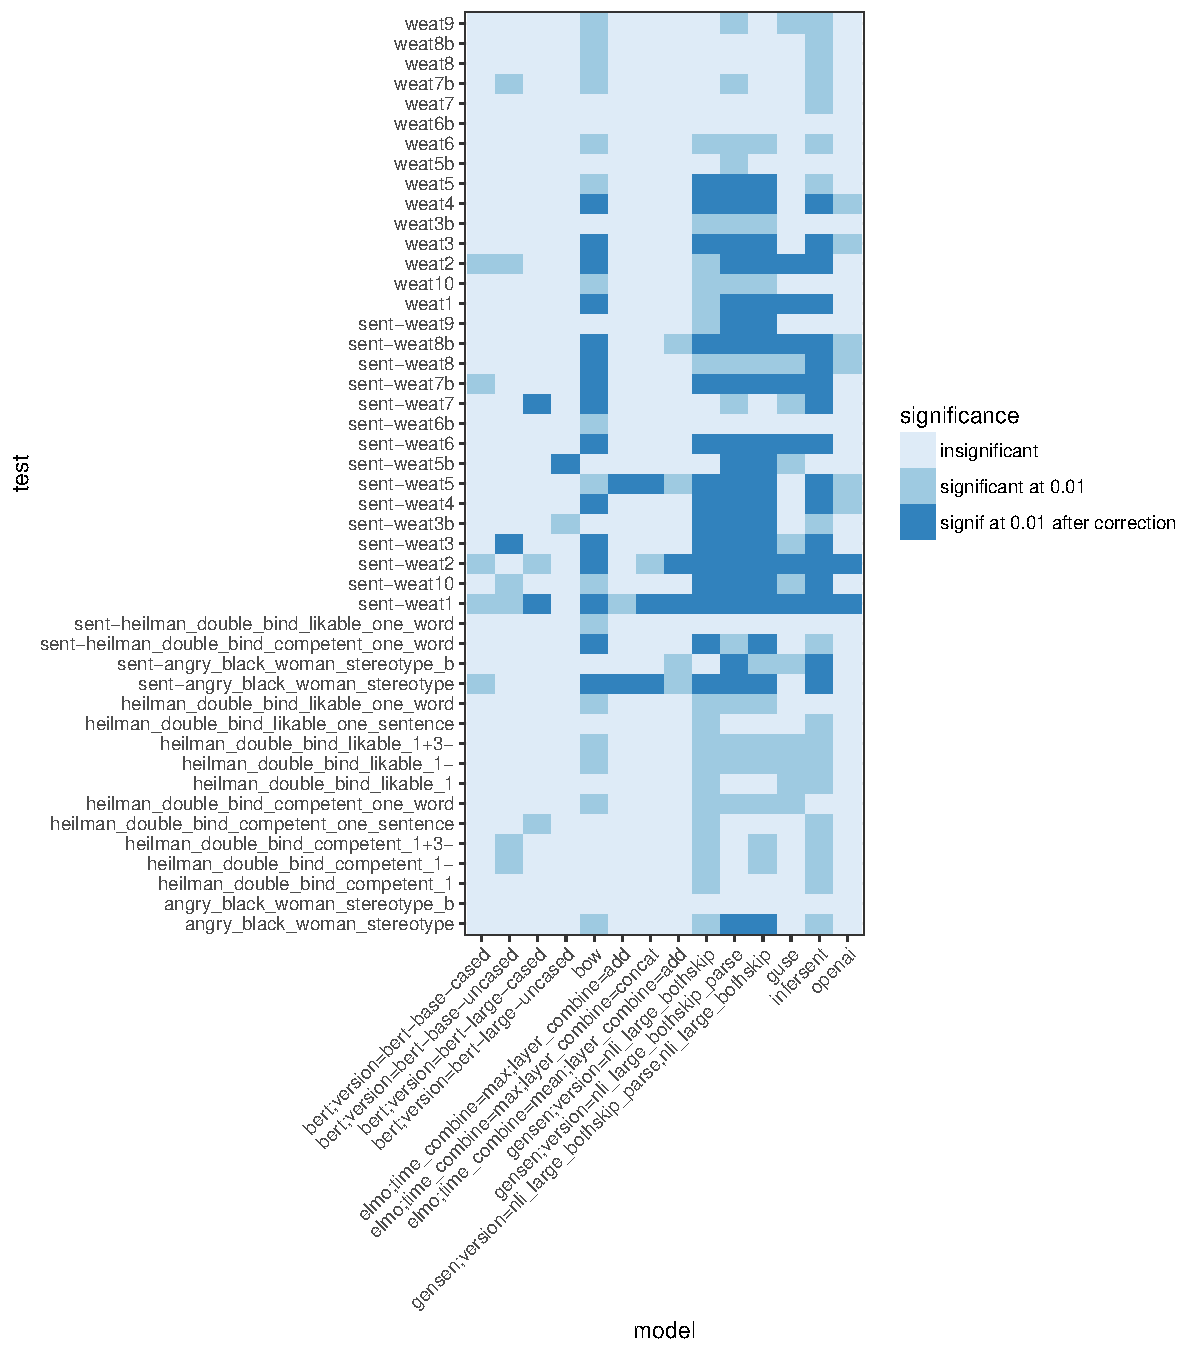
\includegraphics[width=\textwidth]{legend}
	\caption{Significance of results for all models and tests.}
	\label{fig:legend}
\end{figure*}

\end{document}